\subsection{Cross Section and Luminosity}
\label{sec:LumiAndCS}

% Overall, I suggest you rework the first two paragraphs of 2.2 with this in mind.
In this dissertation we are measuring the total and the differential cross section. The cross section in particle physics can be interpreted as area within which an incident particle must appear in order to interact with a scattering center, or, in case of a differential cross section, area $d\sigma$ within which an incident particle must appear to be scattered off by an angle $d\theta$ (Fig.~\ref{fig:CSclassical}). The relashionship between $d\sigma$ and $d\theta$ gives us the expression for a differential cross section $d\sigma/d\theta$. Integrating over $d\theta$, one would get the total cross section $\sigma$. Differentiating $\sigma$ by any kinematic parameter $X$ of the incident particle would give the expression for the differential cross section $d\sigma/dX$.\\

%Why do you discuss the differential cross section with respect to the parameters of the incident particle?
%We are interested instead in the differential cross sections with respect to kinematic parameters
%of the final state particles (it is just in this example the incident particle is the same as the %final state particle).

\begin{figure}[htb]
  \begin{center}
    {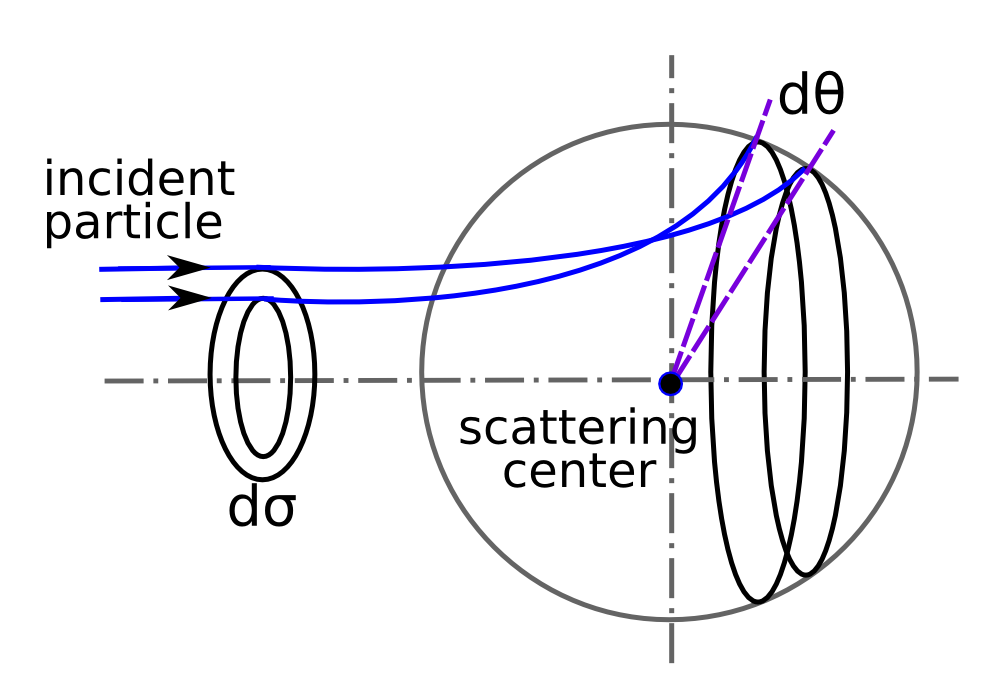
\includegraphics[width=0.70\textwidth]{../figs/WgAbout/CSclassical.png}}
    \caption{Illustration of the differential cross section concept in the classical case.}
    \label{fig:CSclassical}
  \end{center}
\end{figure}

%The first paragraph of 2.2 where you discuss the simplified definition is not easy to read.
%Like "can be interpreted as area within which an incedent particle must appear
%in order to interact”: this is not easy to read at all. Then, other parts of the first
%paragraph can be improved too.
%   The second sentence has several non-trivial ideas and can be split.
However, it is not an actual definition of the cross section but just an illustration of the concept. In fact, the cross section characterizes the probability of two particles to interact \cite{ref_Griffiths}, \cite{ref_Halzen_Martin}, \cite{ref_CS_wiki} or, more specifically, the probability of two particles to interact to produce the specific final state. For example, the probability of a quark and an antiquark to interact to produce a charged lepton, a neutrino and a photon like in our measurement.\\

Referring to the Fig.~\ref{fig:CSclassical}, a number of particles passing through the area $\sigma$ per unit time is $N=L \cdot \sigma$, where $L$ is the number of particles crossing the unit area integrated over a period of time $N$ events occur. Therefore, the cross section $\sigma$ of a specific process $\sigma=N/L$ where N is a number of events of the process occurred. $L$ in this expression refers to the number of the initial state particles and is called the luminosity. \\
  
%Thus, to measure the cross section we need to know total number of events of the given process but we cannot detect events which are out of the detector acceptance or which do not fall satisfy analysis selection criteria. Therefore, the number of events $N$ has to be corrected in a measurement: $N \rightarrow N/(A \cdot \epsilon)$, where $A$ is a detector acceptance and $\epsilon$ is an efficiency of a signal process to pass selection criteria. Other corrections to $N$ may have to be applied depending on the analysis.\\

%The luminosity $L$ is determined based on the collider characteristics. $L$ may not be uniform in time however we are usually interested in measuring the total or differential cross section as a function of a certain kinematic parameter of a final state particle or of a system of final state particles rather than the differential cross section as a function of time and therefore integrate the luminosity over the period of time.\\

% Add more from Griffiths

% what does it mean “to know the phase space”? The expression doesn’t make sense to me.
%Phase space as a term means in the first place the space where dimensions are the four momenta of
%the in and out particles. In what sense do you need to know it to compute the cross section?

To compute a cross section, one has to know the amplitude of the process $M$ and the phase space. The formula of the cross section is called the Fermi's Golden rule \cite{ref_Griffiths}. In case of the scattering of two particles to three final state particles $1+2\rightarrow 3+4+5$, it takes the following form:\\

%Further on, you do mention amplitude several times, but you never explain what it is. You may want to discuss probability amplitudes, connecting initial and final states, etc, with some basic quantum mechanics bra-ket notations, etc.

%You do not need to derive it. But you need to explain, I think, how it comes about and what it means. Just a few more sentences would be enough.

\begin{equation}\label{eq:FermiGoldenRule}
\sigma = \frac{ 1 }{4\sqrt{(p_1p_2)^2-(m_1m_2)^2}} \int |M|^2 (2\pi)^4 \delta^4(p_1+p_2-p_3-p_4-p_5) \prod_{j=3}^{5} \frac{1}{2 \sqrt{\bar{p_j^2}+m_j^2 }}\frac{d^3\bar{p_j}}{(2\pi)^3}  
\end{equation}

where $p_i$ are 4-momenta and ${\bar{p_i}}$ are three momenta of the initial state and the final state particles, $m_i$ are masses of particles.\\ 

The integral over final state kinematics:\\

%The part 470-471, including the equation 27: this doesn’t make sense to me. Maybe Peskin/Shroeder
%can do it, but you shouldn’t. At least not from the start. Even Griffiths with his informal description
%starts with talking about available phase space, then talks about the phase space *factor*, and then
%starts talking about just “phase space”.

\begin{equation}\label{eq:FermiGoldenRule}
\int d \prod_n =  \int (2\pi)^4 \delta^4(p_1+p_2-p_3-p_4-p_5) \prod_{j=3}^{5} \frac{1}{2 \sqrt{\bar{p_j^2}+m_j^2 }}\frac{d^3\bar{p_j}}{(2\pi)^3}  
\end{equation}

is called the phase space \cite{ref_Peskin}.\\

%The calculation of the process amplitude starts with writing the relevant Lagrangian similarly to how it is done in the classical mechanics but in particle physics instead of coordinates we have quantum fields. The Lagrangian allows us to derive the equations of motion however they cannot be solved exactly and, therefore, the perturbative approach is used if coupling constants are $g \ll 1$.\\

%Consider discussing parton luminosity and the cross section expression that involves the PDFs and parton-based cross sections

In case of the proton-proton collisions, we can factorize a cross section of a process $pp \rightarrow P+X$ to a partonic cross section $\sigma(ij \rightarrow P)$ which can be determined using the Fermi's Golden Rule and parton distribution functions $f_i(x_1,Q^2)$ \cite{ref_PDG}, \cite{ref_Lindsey_thesis}:\\

%The paragraph on the lines 473 - 478. I think you need to explain a bit more. Why can we factorize into partonic cross sections? I suggest you refer to the discussion of the proton structure in section 1.4, to the partons and parton PDFs discussed there. You also need to explain what are “i”, “j”, what are x1, x2, etc.

\begin{equation}\label{eq:ppCS_general}
  \sigma(pp \rightarrow P+X)= \sum_{i,j} \int dx_1 dx_2 f_i(x_1,Q^2) f_j(x_2, Q^2) \sigma(ij \rightarrow P).
\end{equation}

%Another question I forgot to mention: in the equation 28 you have Q2. There is no integration over Q2. So what happens to it? Is it that the cross section defined by this equation a function of Q2?

In case of $W\gamma$ process, Eq.~\ref{eq:ppCS_general} takes the following form: \\
%$ij$ can be any $q_1 \bar{q}_2$ pair such that the total charged of $q_1$ and $\bar{q}_2$ equals $\pm 1$.\\

\begin{equation}\label{eq:ppCS_Wg}
  \sigma(pp \rightarrow l \nu_l \gamma + X)= \sum_{i,j} \int dx_1 dx_2 f_i(x_1,Q^2) f_j(x_2, Q^2) \sigma(q_i \bar{q}_j \rightarrow l \nu_l \gamma).
\end{equation}
